\hypertarget{fence-continuous-integration-delivery}{%
\section{Ambiente Fence CID para integração de código}\label{fence-continuous-integration-delivery}}

Principalmente com o desenvolvimento dos \emph{frameworks} \emph{FUnit} e \emph{Fate} para escrita de testes automáticos, constatou-se a necessidade de um ambiente de gerencia automática destes testes. Nesta seção será discutida a solução implementada com integração e entrega contínua, descrevendo de que formas poderia ajudar no processo de trabalho dos desenvolvedores do grupo, como esta solução foi implementada, incluindo seus casos de uso, e a necessidade de aprimoramento para escalabilidade em sistemas distribuídos.

\hypertarget{processo-de-entrega-de-software}{%
\subsubsection{\texorpdfstring{Processo de entrega de software}{Processo de entrega de software}}\label{processo-de-entrega-de-software}}

Ao realizar a entrega de uma nova versão para produção, chamada de \emph{deploy}, uma série de processos são necessários seguindo o processo de trabalho do grupo. Ao estar satisfeito com a nova versão do código desenvolvido, o desenvolvedor realiza um \emph{merge request} para a \emph{branch} \emph{stage} pelo \emph{git}, e quando aprovado, se torna necessário realizar um \emph{deploy} para o ambiente de mesmo nome \emph{stage}, que se trata de um ambiente que reproduz o ambiente de produção, com a motivação de realizar uma verificação final do estado da nova versão antes de ser colocado em produção. Este processo inclui realizar a compilação da aplicação, chamado de \emph{build}, que consiste em vários comandos, como instalação de dependências com o \emph{npm install}, e atualização de \emph{namespaces} com o \emph{composer dump-autoload}.

No processo de trabalho antigo, esta verificação em \emph{stage} era feita de forma manual pelo desenvolvedor. Além disso, caso o desenvolvedor quisesse realizar testes automáticos, o próprio tinha que verificar se os ambientes de execução da \emph{FUnit} e \emph{Fate} estavam adequados e atualizados. No fim, o processo poderia levar uma quantidade significativa de tempo, o qual o desenvolvedor não possuía disponível, especialmente em casos de correções críticas de erros em produção.

A fim de atender a necessidade de uma verificação geral e rápida, que realizasse o processo de \emph{build} da aplicação, execução de testes a partir desse \emph{build} e finalmente o \emph{deploy} para \emph{stage}, foi proposta o desenvolvimento de um ambiente de integração contínua.

\hypertarget{integracao-continua-de-código}{%
\subsubsection{Integração contínua de código}\label{integracao-continua-de-código}}

Nomeado de \emph{Fence Continuous Integration \& Delivery}, ou simplesmente \emph{Fence CID}, esta solução atua na integração do código dos desenvolvedores do grupo, executando as ações necessárias no controle de qualidade quando ocorrem mudanças na plataforma \emph{Gitlab}, o hospedeiro \emph{git} escolhido pelo grupo para controle de versão.

O \emph{Fence CID} foi implementado a partir do \emph{~GitLab Continuous Integration \& Delivery}, disponível automaticamente para qualquer repositório desenvolvido usando \emph{Gitlab}. Com o \emph{Gitlab CI/CD} é possível monitorar diferentes etapas no controle de versão do código, podendo atribuir tarefas de acordo com cada etapa, e no final realizar o processo de \emph{deploy}. No caso do grupo, dois fluxos de execução principais, \emph{pipelines}, foram desenvolvidos, sendo uma para o repositório \emph{git} do \emph{framework} \emph{Fence} e a outra para o repositório \emph{Atlas}, que contém a aplicação com os sistemas que fazem uso do \emph{Fence}. Cada \emph{pipeline} executa os respectivos \emph{jobs} necessários para seu cumprimento, podendo estes serem executados em série ou em paralelo, de acordo com a etapa definida em cada \emph{job}. Na ausência de erros após a execução dos \emph{jobs}, a \emph{pipeline} é qualificada como bem-sucedida.

A descrição de \emph{jobs} e da própria \emph{pipeline} é definida por meio de arquivos de configuração \emph{YAML}, que serão utilizados pelo \emph{Gitlab CI/CD}. Semelhante aos arquivos \emph{JSON}, arquivos \emph{YAML} permitem a serialização de dados por meio de conceitos como escalares, sequências, mapeamentos e âncoras.

Um ponto importante no uso do \emph{Gitlab CI/CD} é a alocação de máquinas disponíveis para executar as \emph{pipelines}. Para uma máquina se tornar disponível é necessário que possua o \emph{Gitlab Runner} instalado, que se trata de um binário capaz de executar as tarefas recebidas pelo servidor principal do \emph{Gitlab CI}. Atribuindo \emph{tags} aos \emph{Gitlab Runner} é possível diferenciar quais máquinas se responsabilizarão por quais tarefas.

\hypertarget{funcionamento-de-uma-pipeline}{%
\subsubsection{\texorpdfstring{Funcionamento de uma \emph{pipeline}}{Funcionamento de uma pipeline}}\label{funcionamento-de-uma-pipeline}}

Ao abrir ou concluir um \emph{merge request} no repositório \emph{Fence}, se dá início à execução do \emph{pipeline}, como exposta na figura \ref{fig:pipeline}. Pode-se observar a existência da \emph{pipeline} com três estágios definidos, sendo eles o \emph{Build}, o \emph{Test} e o \emph{Deploy}. Cada estágio possui apenas um \emph{job}, significando que toda a \emph{pipeline} é executada em série, sem paralelismo. Por exemplo o \emph{job} \emph{unit test}, responsável pelos testes unitários da \emph{Funit}, será executado apenas se o \emph{job} anterior, \emph{build}, tiver sido realizado com sucesso, notificando os desenvolvedores por e-mail e \emph{Slack} caso contrário.

\begin{figure}[H]
    \centering
    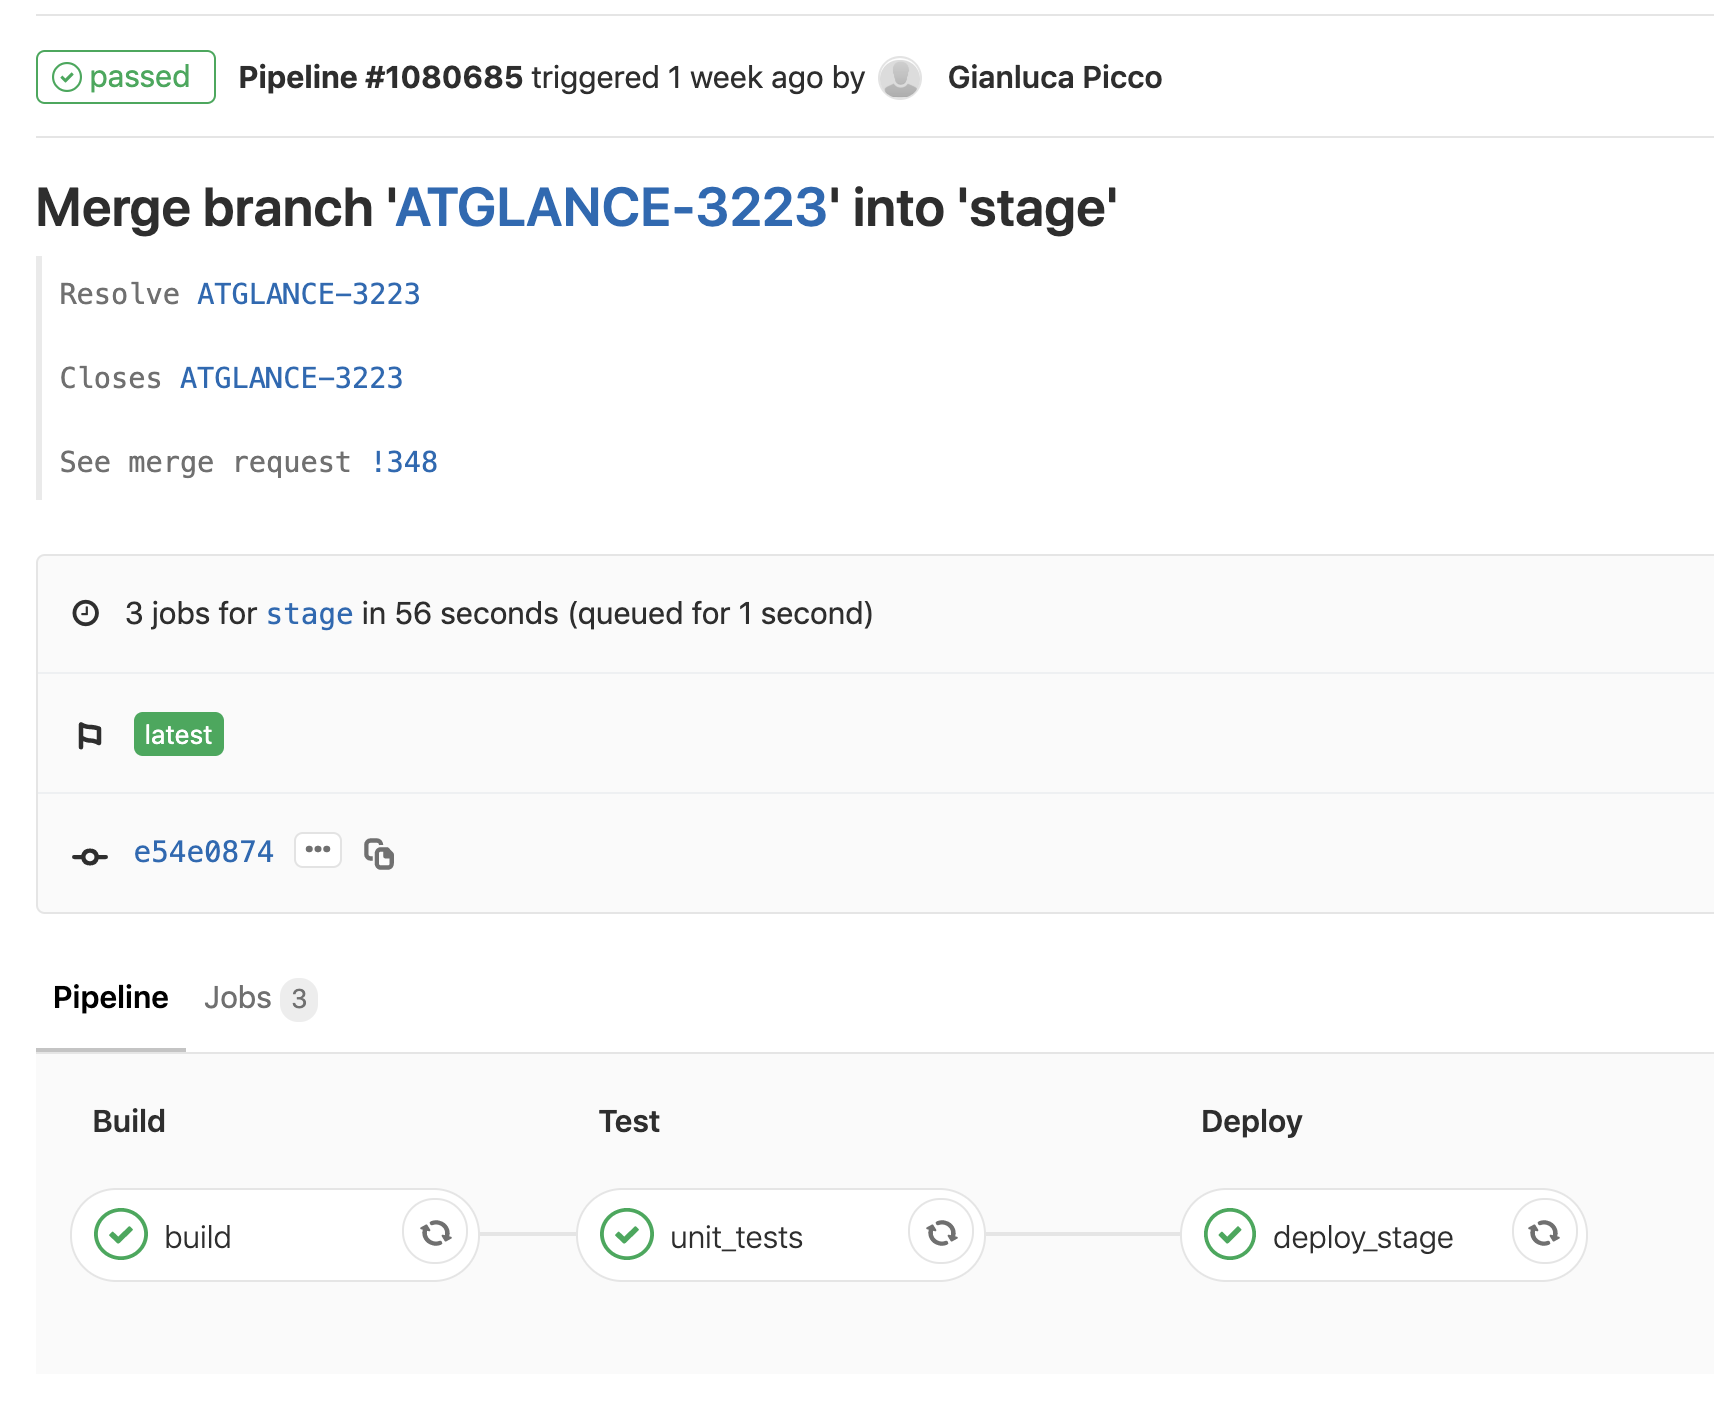
\includegraphics[width=13cm]{source/4-solucao/images/pipeline.png}
    \caption{Exemplo de execução de uma \emph{pipeline}, contendo os \emph{jobs} \emph{build}, \emph{test} e \emph{deploy}.}
    \label{fig:pipeline}
\end{figure}

Entrando no universo do código, na figura \ref{fig:pipeline-2}(a) tem-se o detalhamento do \emph{job} \emph{build} no arquivo \emph{YAML}. Decompondo o arquivo de acordo com seus parâmetros, é possível compreender seu funcionamento. \emph{Stage} define a etapa em que o \emph{job} será executado na \emph{pipeline}, como na etapa \emph{Build} de mesmo nome. Em \emph{only} são definidas as condições para execução do \emph{job}, que neste caso ocorre apenas em \emph{merge requests}. O parâmetro \emph{tags} se responsabiliza em definir quais máquinas podem executar o \emph{job}, que neste caso é o servidor de \emph{stage} dos sistemas. Por fim têm-se \emph{before\_script} e \emph{script}, os quais contêm a lógica a ser executada pelo \emph{job}, sendo neste exemplo os passos necessários para compilação.

Da mesma forma que feita em \emph{build}, um arquivo de configuração é escrito para cada \emph{job} a ser executado. \emph{Gitlab CI/CD} permite a utilização de configurações avançadas nestes arquivos, que foram amplamente utilizadas na construção das \emph{pipelines} do projeto, como extensão de parâmetros, disponibilidade de variáveis globais durante a execução da \emph{pipeline} e repetição do \emph{job} em caso de falha. Por fim, os arquivos de configuração são unificados em um arquivo único, chamado \emph{gitlab-ci.yml} e ilustrado na figura \ref{fig:pipeline-2}(b), que será automaticamente lido pelo \emph{Gitlab CI/CD}.

\begin{figure}[H]
    \centering
    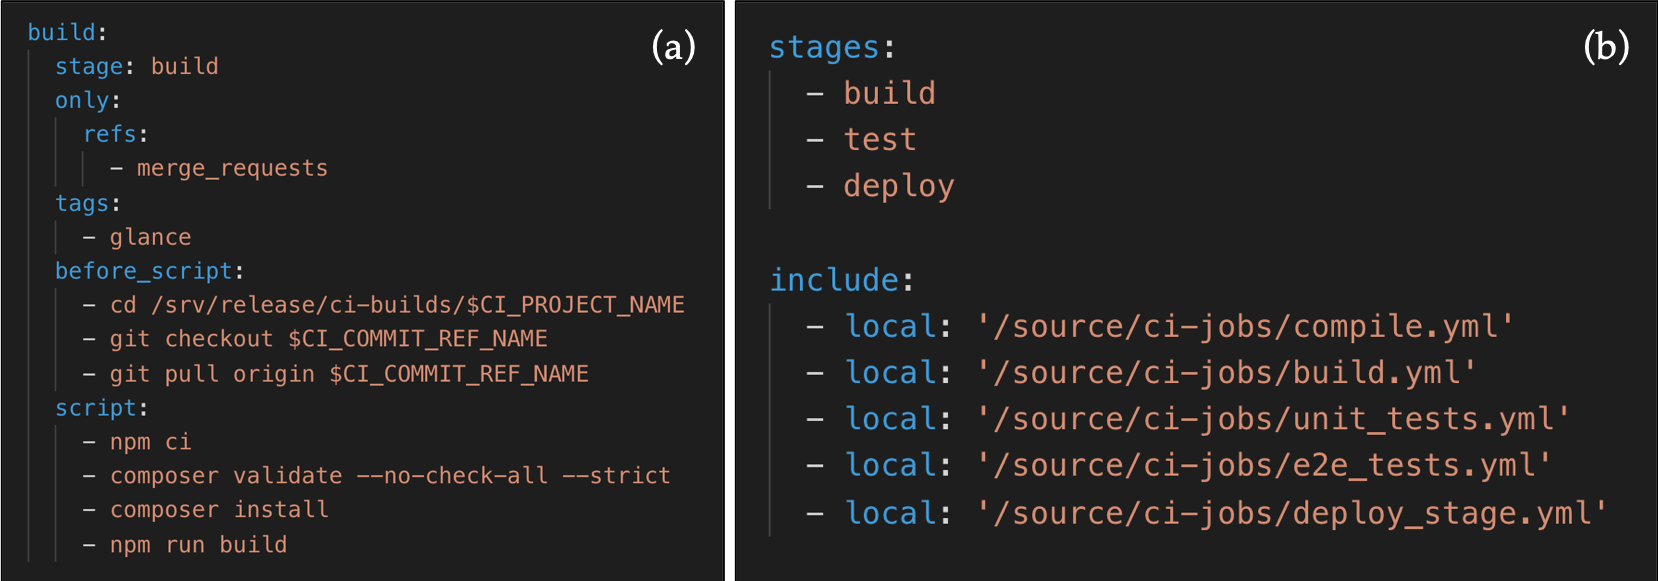
\includegraphics[width=15cm]{source/4-solucao/images/pipeline-2.png}
    \caption{Arquivo de configuração do \emph{job} \emph{build} em $(a)$ e o arquivo principal, da \emph{pipeline}, em $(b)$.}
    \label{fig:pipeline-2}
\end{figure}

No caso do repositório \emph{Atlas} a \emph{pipeline} é bem similar, com algumas ressalvas. Como a aplicação depende do \emph{Fence} para o seu funcionamento, é interessante que a \emph{pipeline} do \emph{framework} seja executada juntamente com a própria, podendo inclusive ser paralelizado. Conforme, como pode ser visto na figura \ref{fig:pipeline-update}, a \emph{pipeline} do \emph{Atlas} invoca a \emph{pipeline} do \emph{Fence} e ambas são executadas em paralelo, rodando os respectivos \emph{jobs} das etapas de \emph{Build} e \emph{Test}. Pode-se notar também a existência do \emph{job} \emph{e2e\_tests}, responsável pela execução do \emph{Fate}. Este \emph{job} está presente apenas no repositório \emph{Atlas} pelo fato do \emph{Fence} ser apenas um \emph{framework} e não possuir interfaces próprias, enquanto o \emph{Atlas}, por ser uma aplicação, dispõe de páginas web.

\begin{figure}[H]
    \centering
    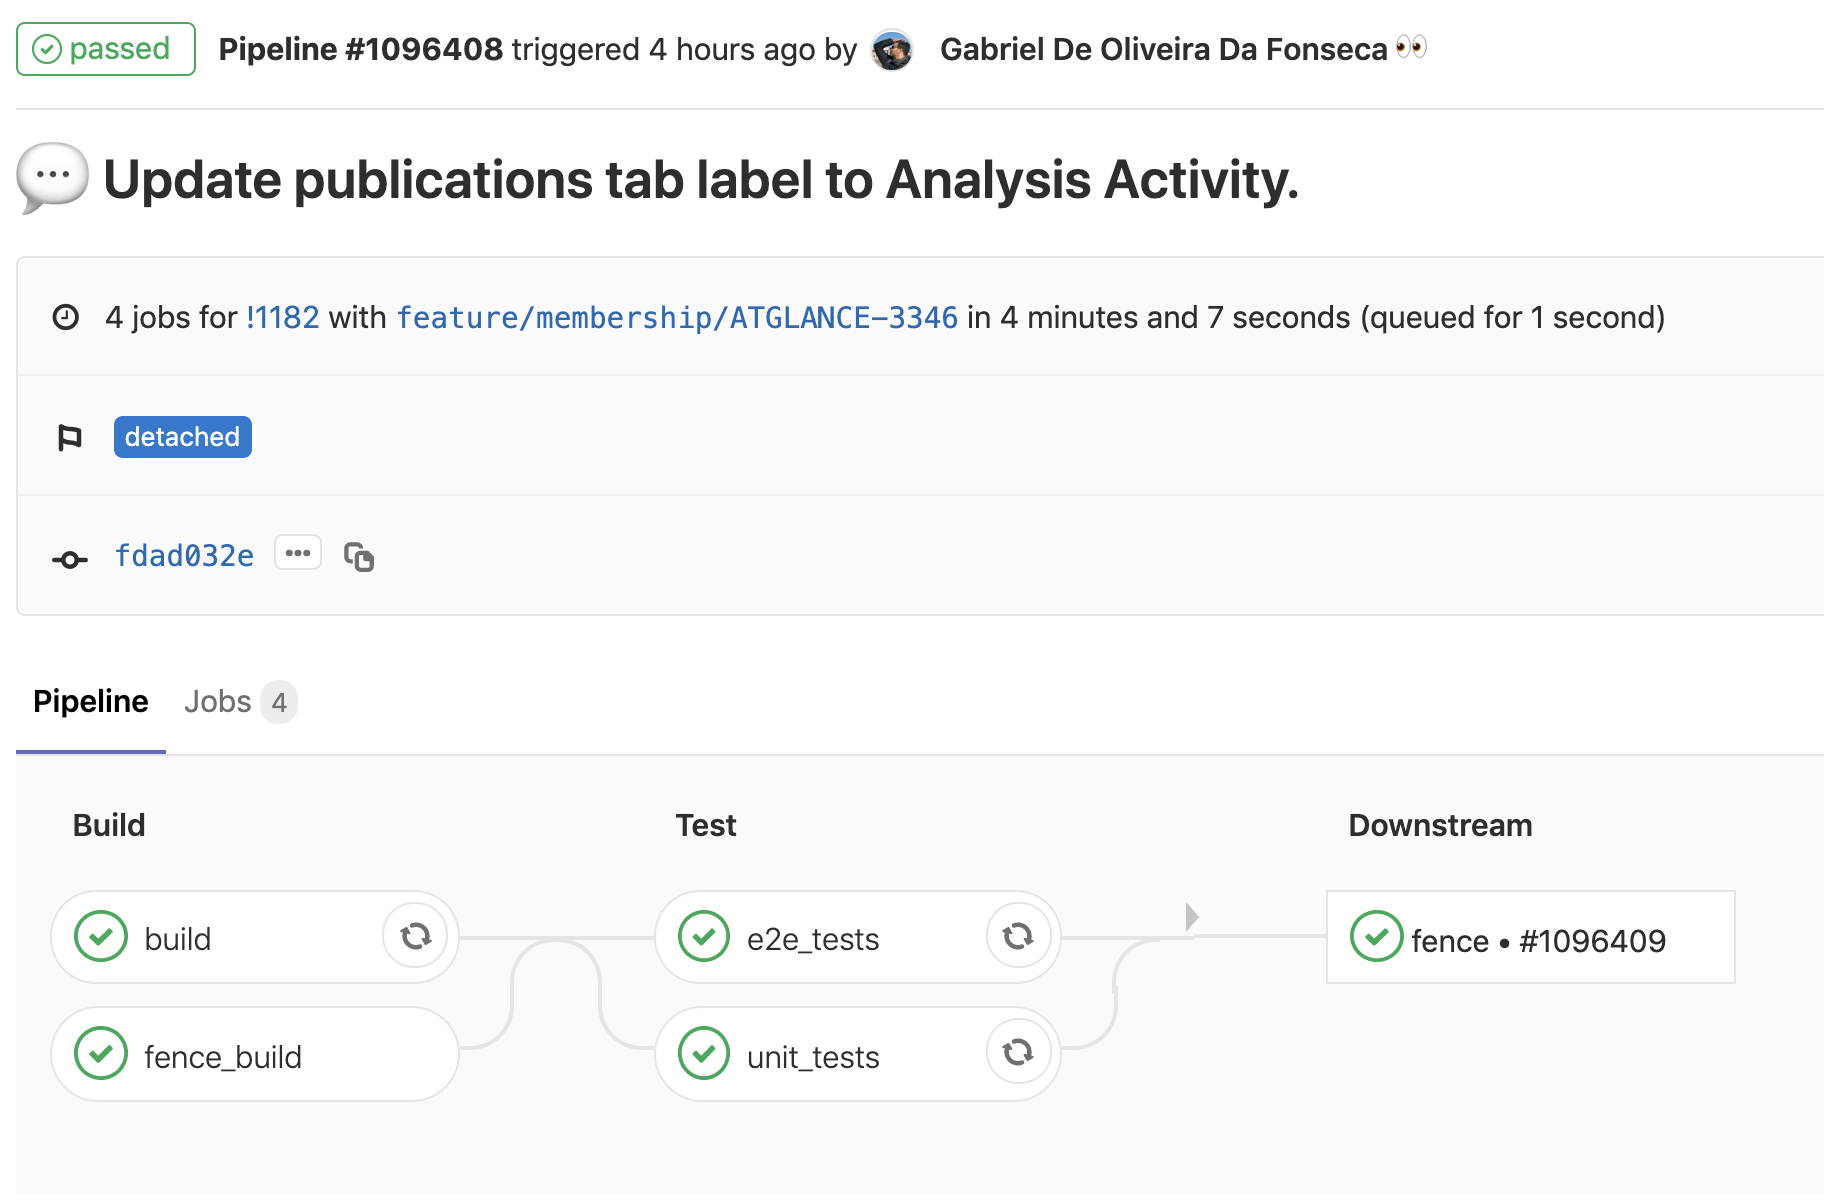
\includegraphics[width=13cm]{source/4-solucao/images/pipeline-update.png}
    \caption{Ilustração da integração entre as \emph{pipelines} do \emph{Atlas} e \emph{Fence}.}
    \label{fig:pipeline-update}
\end{figure}

Implementada a integração e entrega contínua, a atenção voltou-se para outra questão. Como visto anteriormente nesta dissertação, enquanto testes unitários são rapidamente executados dada a sua simplicidade, o acúmulo de testes \emph{e2e} pode gerar lentidão na execução de testes. Por conta disso, um esforço foi feito a fim de paralelizar estes testes, que será abordado na próxima seção.

\hypertarget{orquestracao-em-containers}{%
\subsubsection{\texorpdfstring{Orquestração em \emph{containers}}{Orquestração em containers}}\label{orquestracao-em-containers}}

Ao buscar estratégias para execução de testes em paralelo do \emph{Fate}, alguns desafios foram considerados. Primeiramente, para a execução em paralelo ser possível, seria necessário a disponibilidade de múltiplas instancias de sistemas operacionais , como presente em um \emph{cluster}. Em seguida, essas instancias precisariam ser capazes de executar os testes, contendo todas as ferramentas necessárias. Isso inclui softwares, como \emph{git} e \emph{Nodejs}, e pacotes \emph{npm}, como o \emph{WebdriverIO} e o \emph{Mochajs}. Por fim, essas instancias precisariam se comunicar em si, de forma que fosse balanceado a execução dos testes de forma igualitária. Assim que uma instancia finalizasse a execução de um teste, ela se tornaria disponível para receber outro.

Para a solução da disponibilidade de instancias e máquinas, foi encontrada a possibilidade de utilizar recursos disponíveis pela infraestrutura do \emph{CERN}. Por ser um centro de pesquisas de alto porte, há a disponibilidade de máquinas já integradas com o \emph{Gitlab CI/CD} para serem utilizadas no projeto. Estas máquinas são chamadas de \emph{Runners}, e a figura \ref{fig:e2e-pipeline}(a) mostra um exemplo exibindo-as na interface do \emph{Gitlab}.

Em relação a questão do ambiente das máquinas, a solução encontrada foi a adoção do \emph{Docker}. \emph{Docker} é uma plataforma famosa na comunidade, onde se torna possível a hospedagem de aplicações em um ambiente isolado, chamado de \emph{container}, em que o desenvolvedor consegue empacotar o software de maneira padronizada. A plataforma possui uma performance superior a virtualização convencional e permite configurar diferentes ambientes com facilidade a partir do conceito de imagens, no qual é possível gerar um \emph{container} a partir da representação de um outro \emph{container} já existente. Isso permite o ambiente de uma aplicação ser mais modularizado e escalável.

Para começar a utilizar \emph{Docker} um arquivo \emph{Dockerfile} foi gerado para o repositório \emph{Fate}, como ilustrado na figura \ref{fig:e2e-pipeline}(b), contendo os comandos de instalação para as dependências do \emph{framework}. É então construída uma imagem a partir destes comandos, que é enviada para o repositório central de imagens \emph{docker} do \emph{CERN}. Esta imagem fica então disponível para outros repositórios hospedados no \emph{Gitlab} poderem utilizar.

Uma \emph{pipeline} foi implementada no caso do \emph{Fate} , como pode ser visto na figura \ref{fig:e2e-pipeline}(c), em que é realizada uma verificação do próprio funcionamento do \emph{framework} quando são desenvolvidos novos testes \emph{e2e}. Estes testes, juntamente com os anteriores, são compilados e testados diversas vezes para garantir sua robustez. Sendo o resultado bem-sucedido, a imagem \emph{docker} do \emph{Fate} é atualizada e seu \emph{upload} feito, podendo ser utilizada nos futuros \emph{jobs} de \emph{e2e tests} da \emph{pipeline} do repositório \emph{Atlas}. Pode-se dizer que o \emph{Fate} testa os seus próprios testes.

\begin{figure}[H]
    \centering
    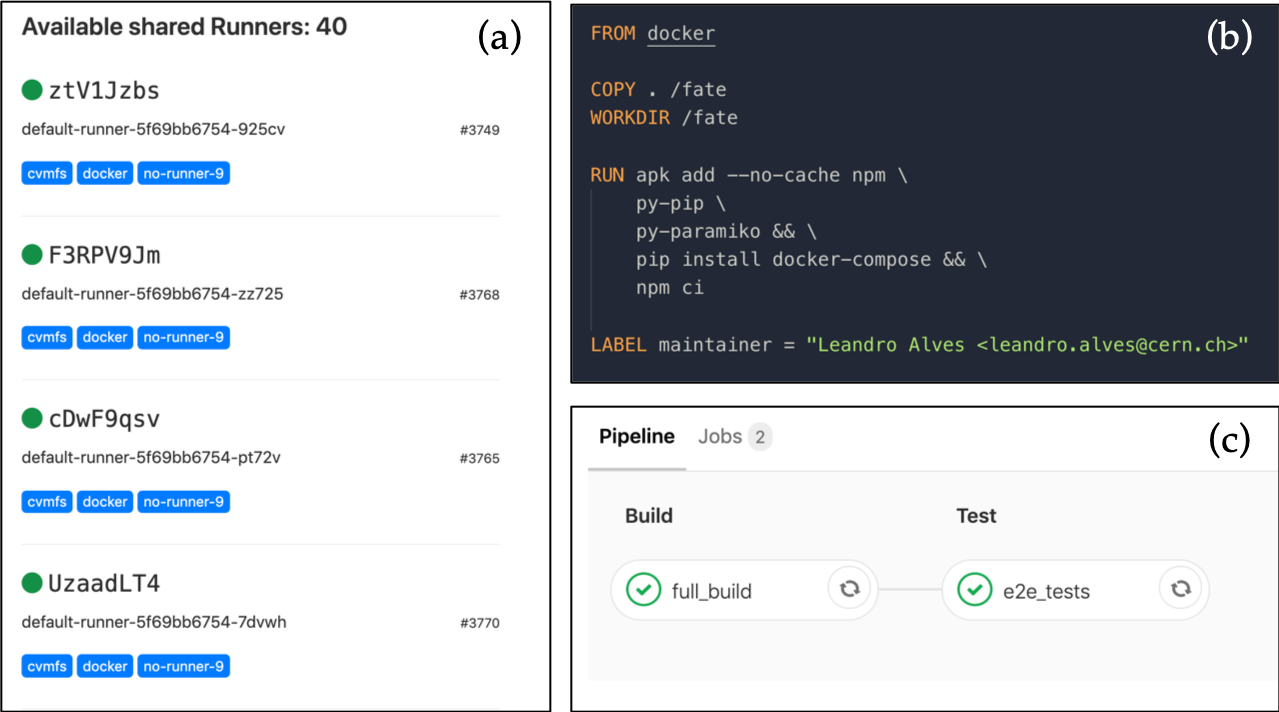
\includegraphics[width=15cm]{source/4-solucao/images/e2e-pipeline.png}
    \caption{Em $(a)$, lista de instancias disponíveis. Em $(b)$, exemplo de arquivo \emph{Dockerfile} para geração de uma imagem. Em $(c)$, a \emph{pipeline} do \emph{Fate}.}
    \label{fig:e2e-pipeline}
\end{figure}

Obtendo as instancias necessárias e um método eficiente de prepará-las, o desafio final passa a ser a intercomunicação e administração destes containers. Para solucioná-lo, foi necessário utilizar em conjunto a ferramenta de orquestração \emph{docker swarm}, o utilitário \emph{docker compose} de configuração \emph{multi-container}, e por fim o \emph{Selenium Grid} para alocação dos testes entre os \emph{containers}.

O \emph{Selenium Grid} faz parte da família \emph{Selenium}, juntamente com o \emph{Selenium Webdriver} e o \emph{Selenium IDE}, e permite a organização e preparação de diversas máquinas para execução testes. Por meio do conceito de \emph{hub} e \emph{nodes}, o \emph{Selenium Grid} define uma máquina central, o \emph{hub}, que será a responsável por gerenciar as máquinas que irão executar os testes, os \emph{nodes}. O \emph{hub} recebe o conjunto de testes a serem executados, acompanhado das informações de execução de cada teste, como por exemplo o sistema operacional ou navegador. A partir disso, o \emph{hub} avalia a configuração de cada \emph{node} presente na malha e aloca os testes conforme a disponibilidade dos \emph{nodes} compatíveis com cada teste. Os comandos provenientes do \emph{Fate} com o \emph{WebdriverIO} são então enviados do \emph{hub} para o \emph{node}, que os executa e informa de volta para o \emph{hub}. Finalizados todos os testes, o \emph{hub} sintetiza os resultados para o \emph{Fate}, o qual gera o relatório para a \emph{pipeline}.

Para implementar essa arquitetura no projeto, foram utilizadas imagens \emph{docker} oficiais do \emph{Selenium Grid}. Estas imagens são \emph{selenium/hub}, \emph{~selenium/node-chrome} e \emph{~selenium/node-firefox}, tornando disponível para teste os navegadores \emph{Chrome} e \emph{Firefox}, que são os mais populares pelos usuários dos sistemas. \emph{Docker compose} é utilizado para dar as instruções de geração destas imagens, como por exemplo que portas serão utilizadas por cada \emph{container}, sua ordem de construção, variáveis de ambiente, e o número de \emph{containers} que serão implementados a partir de cada imagem. Todas estas instruções são definidas no arquivo \emph{docker-compose.yml}, como ilustrado na figura \ref{fig:containers}, que é então utilizado pelo \emph{docker swarm} para finalmente implementar múltiplos \emph{containers} a partir dos \emph{Runners} disponíveis no \emph{Gitlab CI/CD} do \emph{CERN}.

\begin{figure}[H]
    \centering
    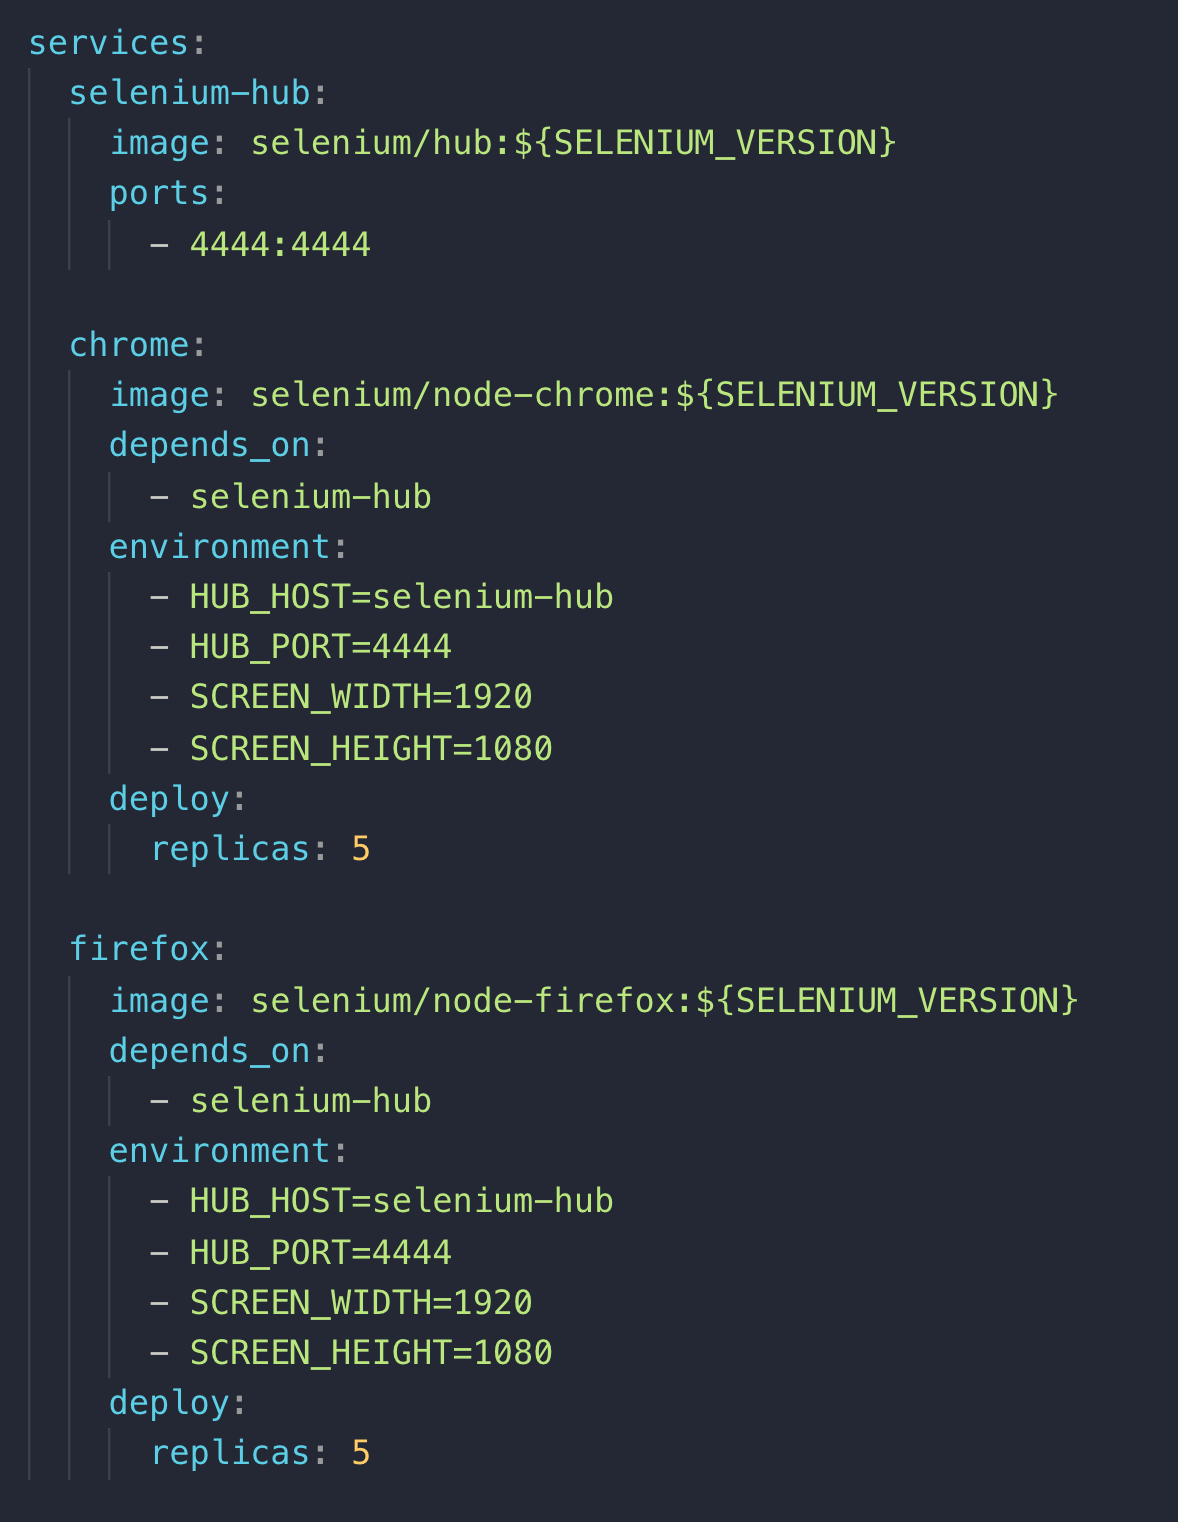
\includegraphics[width=11cm]{source/4-solucao/images/containers.png}
    \caption{Arquivo de configuração do \emph{docker compose}, contendo o balanceamento ente \emph{hub} e \emph{nodes}.}
    \label{fig:containers}
\end{figure}

De forma resumida, no \emph{job} \emph{e2e tests} é utilizada a imagem \emph{docker} do \emph{Fate} que possui as instruções do orquestrador \emph{docker compose}. Estas instruções são interpretadas e múltiplos \emph{containers} são implementados a partir da disponibilidade de máquinas no \emph{Gitlab CI/CD}. Estes \emph{containers} fazem parte da rede do \emph{Selenium Grid} que os dividem entre \emph{hub} e \emph{nodes}. O \emph{container} \emph{hub} gerência as execuções dos testes nos \emph{nodes} e por fim coleta os resultados, que serão enviados no final para a \emph{pipeline}.
